% !TEX root = ../disertace.tex
%!TEX encoding = UTF-8 Unicode

\chapter{Annotation}
\label{sec:annot}

\section{Annotation process}
\label{sec:annot:how}
\todo pozor, neco o tom, jak se anotovalo, je v uvodu \Sref{sec:annot:analysis}. \\
Takze s nastrojem a daty predanotovanymi dle Hnatkove jsme postupovali takto: rozdeleni na davky, podle toho, jak jsme doplnovali nove predanotace, ale take abychom mohli zkoumat vliv ruznych postupu v anotaci na kvalitu vyslednych dat (neco malo hotovo, ale jinak future work). 

Put the table from wiki here.





%%%%%%%%%%%%%%%%%%%%%%%%
\section{Basic quantitative characteristics of the annotations}
\label{sec:annot:what}

\begin{table}[htdp]
\begin{tabular}{l|r|r|r|r|r|r}
 parallel annotations  & 1    & 2    & 3   & PDT    & 2+3$/$PDT & *$/$PDT \\
 \hline
 t-files & 1288   & 1412   & 465   & 3165   & 59\%        & 100\% \\
 t-nodes & 248448 & 343834 & 82683 & 674965 & 63\%        & 100\% \\
\end{tabular}
\caption{How much data was annotated by 1, 2, or 3 annotators in parallel; compared to the size of PDT (t-data). The last collumn just indicates that we have indeed annotated all the data of PDT 2.0 t-layer.}
\label{tab:parallel-anot}
\end{table}%





%%%%%%%%%%%%%%%%%%%%%%%%
\section{Pre-annotation}
\label{sec:annot:pre}
Because MWEs tend to occur repeatedly in a text, we have decided to test pre-annotation both for speed improvement and for improving the consistency of annotations. 
%We work o
We use an assumption that \emph{all occurrences of a MWE share the same tectogrammatical tree structure}. We can call this assumption \emph{``One tree per MWE,''} and view it as a modification of famous assumption ``One sense per collocation'' of \citet{yarowsky:1993}. In the surface representation of the MWE, there are \emph{no restrictions on the word order} other than those imposed by the tree structure itself. Our assumption is however more inspired by an idea of \citet{holub-bohmova:2000:RANLPIR}, who proposed to use so called ``Dependency microcontext structures (DMCS)'' in information retrieval. DMCS were inspired by tectogrammatical tree structures, but modified a bit for easier extraction and handling. In contrast, we use tectogrammatical structures as they are. What impact it has for instance in relation to coordinations can be seen in \todo\ \Sref{}. For the analysis of results of our assumption see \todo.

We employed four types of pre-annotation, only some of wich are based on the above assumption:

\begin{enumerate}[A)]

\item \label{pre-hnatkova}External pre-annotation provided by Milena Hnátková (see~\citealp{hnatkova:2002}). With each MWE a set of rules is associated that limits possible forms and surface word order of parts of a MWE. This approach was devised for corpora that are not syntactically annotated and is very time consuming.

\item \label{pre-static}Our one-time pre-annotation with those MWEs from SemLex that have been previously used in annotation, and as a result of that, they already have a tree structure as a part of their entry.

\item \label{pre-on-load}Dynamic pre-annotation as in \ref{pre-static}, only with the SemLex entries that have been recently added by an annotator. 

\item \label{pre-on-annot}When an annotator tags an occurrence of a MWE in the text, other occurrences of this MWE in the article are identified automatically.

This is exactly what happens:
	\begin{enumerate}[1)]
	\item Tree structure of the selected MWE is identified via \ntred
	\item The tree structure is added to the MWE's entry in SemLex
	\item All the sentences in the given file are searched for the same MWE using its tree structure (via  \ntred)
	\item Other occurrences returned by  \ntred\ are tagged with this MWE's ID, but these occurrences receive an additional attribute ``auto'', which identifies them (both in the s-files and visually in the annotation tool) as annotated automatically.
	\end{enumerate}

\end{enumerate}

Pre-annotation (\ref{pre-hnatkova})~was executed once for all of the PDT. (\ref{pre-static})~is performed each time we merge MWEs added by annotators into the main SemLex. We carry out this annotation in one batch for all PDT files remaining to annotate. (\ref{pre-on-load})~is done for each file while it is being opened in the annotation environment. 
(\ref{pre-on-annot})~happens each time the annotator adds a new MWE into SemLex and uses it to annotate an occurrence in the text. In subsequent files instances of this MWE are already annotated in step (\ref{pre-on-load}), and later even in (\ref{pre-static}).
%, when the lexia (lexicon entry) is merged into the main SemLex. 
 
%\xxx{PRO FUTURA
%We have currently performed double blind annotation of a part of data without pre-annotation (\ref{pre-static}) and (\ref{pre-on-load}). We also have smaller samples annotated without any pre-annotation and only with pre-annotation (\ref{pre-hnatkova}). Analysis of this data is necessary  to show that our assumption is correct and all the occurrences of a lexia share the same tree structure. Then we can safely add remaining pre-annotation steps. Provided the inter-annotator agreement is good enough we can also stop our current (rather expensive and time consuming) practice of double annotation of each file and comparing the annotations.} % end XXX

After the pilot annotation without pre-annotation (\ref{pre-on-annot})  we have compared instances of the same tags and found that 10.5\% of repeated MWEs happened to have two different tree representations. Below we analyse several most important sources of these inconsistent t-trees and possible improvements:
\begin{itemize}
%
\item \emph{Occasional lemmatisation errors.} They are not very frequent, but there is no efficient way to find and correct them before the annotations. So there is not much we can do but it is not very important. Our annotations can however serve as a source for automatic corrections.
	\begin{itemize}
	\item \textit{jižní Korea {\rm vs.} Jižní Korea} (southern vs. South Korea)
	\end{itemize}
% chyba anotatora (neoznaci v LexSemAnnu slovo)
\item \emph{Annotator's mistake (not marking correct words).} When an annotator makes an error while marking a first occurrence of a MWE, the tree representation that gets stored in SemLex is incorrect. As a result, pre-annotation gives false positives or fails to work. 

It is therefore necessary to allow annotators to correct the tree structure of a SemLex entry, i.e. extend functionality of the annotation tool. Once all the types of pre-annotation are employed, this error can happen only once, because all the following occurrences of a MWE are pre-annotated automatically. We are currently working on these improvements.
%
\item \emph{Gender opposites, diminutives and augmentatives.} These are currently represented by variations of t-lemma. 
We believe that they should be represented by attributes of t-nodes %, which would explicate information that is now given only implicitly. 
that could be roughly equivalent to some of the lexical functions in the Meaning-text theory (see \cite{melcuk:1992}).
This should be tackled in some future version of PDT. Once resolved it would allow us to identify following (and many similar) cases automatically. 
	\begin{itemize}
	\item \textit{obchodní ředitel {\rm vs.} obchodní ředitelka} \\(lit.: managing director-man vs. m. director-woman)
	\item \textit{rodinný dům {\rm vs.} rodinný domek} \\(lit.: family house vs. family little-house; but the diminutive \emph{domek} means basically “family house”)
	\end{itemize}
%
Currently we annotate these cases with the same MWE, but all the instances with the derived variants of t-lemma (like \emph{ředitelka } or \emph{domek} must be identified manually (see Section~\ref{sec:annot:pre}). We had plans to try automatic identification of some diminutives and gender opposites derived by the most common derivation patterns, but annotations were faster than coding, so we never got to it.

%
\item \emph{Newly established t-nodes corresponding to elided parts of MWEs in coordinations.} Since t-layer contains many newly established t-nodes, many of which cannot generate a surface word, our original decision was to hide all of these nodes from annotators and generate for them pure surface sentence. This decision resulted however in the current situation, when some MWEs in coordinations cannot be correctly annotated. 
%It is necessary to elide common part of coordinated multiword lexeme. 
For instance \emph{První a druhá světová válka} (First and Second World War) is a coordination of two multiword lexemes. A tectogrammatical tree that includes it does have newly established t-nodes for “world” and “war” of the first lexeme but they are elided in the surface sentence. 

After analysing annotated examples like the one above we have decided to generate surface words from some of the newly established t-nodes in order to allow correct annotation of all the MWEs. These ``added'' words will be displayed in grey and while some morphological forms of these words may be incorrect, we believe they will serve their purpose.

\xxx{The first lexeme cannot be identified automatically. In this and other similar cases t-nodes for elided parts of multiword lexemes should have been part of PDT, in our opinion. Given that our goal is to have one t-node for each lexia, however, we believe it would not be efficient to invest substantial amount of manual work into adding these elided t-nodes now only to eliminate them more efficiently in near future. We can just as well leave it to our annotators to identify these instances of MWEs (it is as common for NEs, as it is for lexias) manually.}

\item \xxx{\emph{Bridging anaphora} e.g. Ceska narodni banka <- banka \\
Since in the context the second expression stands for the first only with some words ellided, our annotators were instructed to annotate it as an instance of the lexia \emph{Česká národní banka}. 
This problem could be solved by annotations of coreference. If the coreference between nominal expressions was present in the PDT 2.0, our annotators would simply mark the first occurence and all the anaphoric expressions would be marked automatically. 
} % end xxx
\end{itemize}


\xxx{
\emph{spojit s 'itemize' vyse!}\\
because these cases are caused by ellipses, variations in lexical form such as diminutives etc., or wrong lemmatisation, rather than inconsistencies in the tree structure. These cases show us some problematic issues in PDT 2.0, for instance:
\begin{itemize}
\item \textit{jižní Korea {\rm vs.} Jižní Korea} \\(southern vs. South Korea) -- wrong lemmatisation
\item \textit{obchodní ředitel {\rm vs.} obchodní ředitelka} \\(lit. managing director-man vs. m. director-woman) -- in future these should have one t-lemma. Morphological gender should be specified by an attribute of a t-node.
\end{itemize}
} % end xxx


Up to now we have not found any MWE such that its structure cannot be represented by a single tectogrammatical tree. 1.1\% of all occurrences were not connected graphs, but this happened due to errors in data and to our incorrect handling of coordinations with newly established t-nodes (see above). This corroborates our assumption that (disregarding errors) all occurrences of a MWE share the same tree structure. As a result, we started storing the tree structures in the SemLex entries and employ them in pre-annotation (\ref{pre-on-annot}). This also allows us to use pre-annotations (\ref{pre-static}) and (\ref{pre-on-load}), but we have decided not to use them at the moment, in order to be able to evaluate each pre-annotation step separately. Thus the following section reports on the experiments that employ pre-annotations (\ref{pre-hnatkova}) and (\ref{pre-on-annot}).





%%%%%%%%%%%%%%%%%
\section{Measuring the inter-annotator agreement}
\label{sec:annot:analysis}
During the annotations we employed four annotators. Three of them annotated a significant amount of work, the fourth, who is not mentioned elswhere in this text, helped with various experiments. The annotator identified by name $sta$ replaced annotator $sid$, while $vim$ worked with us during whole course of the project. 

Below we 

The ratio of general named entities versus SemLex entries was approx. 52:48 for annotator $sid$ and 50:50 in the case of annotator $vim$. This, and some other comparisons are given in Table~\ref{tab:anot}. Both of them annotated 1090 files in parallel. The data consisted of  350,177 tokens representing 284,029 t-nodes.

\begin{table}[h]
\centering
\begin{tabular}{l|r|r}
type of MWE&$sid$&$vim$\\
\cline{1-3}
SemLex entries -- instances&9,427&9,477\\
 - total entries used&4,472&4,067\\
Named Entities&10,208&9,621\\
 - address & 20 & 2 \\
 - biblio & 4 & 14 \\
 - foreign & 83 & 50 \\
 - institution&2,344&1,928\\
 - location&619&700\\
 - object&1,046&1,299\\
 - other&1,188&1,498\\
   - person/animal&3,246&3,232\\
      - time&1,658&898\\

\end{tabular}
\caption{Annotated instances of significant types of MWEs by annotators $sid$ and $vim$}
\label{tab:anot}
\end{table}


\subsection{The measure}
\label{agreement}

In this section our primary goal is to assess whether with our current methodology we produce reliable annotations of MWEs. To that end we measure the amount of inter-annotator agreement that is above chance. Our attempt exploits {\it weighted kappa measure} $\kappa_w$ \cite{cohen:1968}.

The reason for using a weighted measure is essential for our task: we do not know which parts of sentences are MWEs and which are not. Therefore annotators work with all words and even if they do not agree on the type of a particular MWE, it is still an agreement on the fact that this t-node is a part of some MWE and thus should be tagged. This means we have to allow for partial agreement on a tag.

There are, however, a few sources of complications in measuring agreement of our task even by $\kappa_w$:
\begin{itemize}
	\item % castecne pruniky tagu
	Each tag of a MWE identifies a subtree of a tectogrammatical tree (represented on the surface by a set of marked words). This allows for partial agreement of tags at the beginning, at the end, but also in the middle of a surface interval (in a sentence). Instead, standard measures like $\kappa$ assumes fixed, bounded items, which are assigned some categories.
	\item % nejasny pocet tagu
	There is no clear upper bound as to how many (and how long) MWEs there are in texts. Cohen's $\kappa_w$ counts agreement on known items and these are the same for both annotators. On the other hand, we want to somehow count agreement on the fact, that given word is not a part of MWE.
% [to sem nepatri, leda pouzit jinde] Since the disagreement in $\kappa$ is substracted from one and one is unreachable,\footnote{Let say that both annotators say some word is not part of a MWE, we treat it like an agreement..........} we should use another upper bound.
	\item 
	There is not a clear and simple way to estimate the amount of agreement by chance, because it must include the partial agreements mentioned above.
\end{itemize}

Since we want to keep our agreement calculation as simple as possible but we also need to take into account the issues above, we have decided (as mentioned above) to start from $\kappa_w$ as defined in \cite{artstein:2007}: $\kappa_w = 1 - \frac{D_o}{D_e} = \frac{A_o - A_e}{1 - A_e}$ (explanation in Equation \ref{ourkappa}) and to make a few adjustments to allow for an agreement on non-annotation and an estimated upper bound. We explain these adjustments in following paragraphs on the example of paralled data of annotators $sid$ and $vim$\footnote{The same calculations are done for our other pair: $sta$ and $vim$.} and we summary quantitative data for this pair in Table~\ref{tab-agreement}.

Because we do not know how many MWEs there are in our texts, we need to \textit{calculate the agreement over all t-nodes}, rather than just the \mbox{t-nodes} that ``should be annotated''. This also means that the theoretical maximal agreement (upper bound) $U$ cannot be 1. If it was 1, it would be saying that all nodes are part of MWEs. 

Since we know that $U < 1$ but we do not know its exact value, we use the \textit{estimated upper bound} $\widehat{U}$ (see Equation \ref{eq-upper-bound}). Because we calculate $\widehat{U}$ over all t-nodes, we need to account not only for agreement on tagging a t-node, but also for agreement on a t-node not being a part of a MWE, i.e. not tagged at all. 
%
%\footnote{If we did not do this, there would be no difference between t-nodes, that were not tagged (annotators agreed they are not a part of a MWE) and the t-nodes that one annotator tagged and the other did not (i.e. they disagreed).}
%
This allows us to positively discriminate the cases where annotators agree that a t-node is not a part of a MWE from the cases where one annotator annotates a t-node and the other one does not, which is evidently worse.

%\newpage
If $N$ is the number of all t-nodes in our parallel data and $n_{A \cup B}$ is the number of t-nodes annotated by at least one annotator, then we estimate $\widehat{U}$ as follows:
\begin{equation}
\label{eq-upper-bound}
\widehat{U} = \frac{n_{A \cup B}}{N} + 0.051 \cdot \frac{N - n_{A \cup B}}{N}= 0.213.
\end{equation}

The weight $0.051$ used for scoring the t-nodes that were not annotated is explained below ($c=4$). Because $\widehat{U}$ includes all the disagreements of the annotators, we believe that the real upper bound $U$ lies somewhat below it and the agreement value 0.213 is not something that should (or could) be achieved. It is however based on the assumption that the data we have not yet seen have similar proportion of MWEs as the data we have used for the upper bound estimate.

To account for partial agreement we divide the t-nodes into 5 classes $c$ and assign each class a weight $w_c$ as follows: 

\begin{enumerate}[$c=1$]
\item
If the annotators agree on the exact tag from SemLex, we get maximum information: $w_1 = 1$.
\item
If they agree that the t-node is a part of a NE or they agree that it is a part of some entry from SemLex, but they do not agree which NE or which entry, we estimate we get about a half of the information compared to when $c=1$: $w_2 = 0.5$.
\item
If they agree that the t-node is a part of a MWE, but disagree whether a NE or an entry from SemLex, it is again half the information compared to when $c=2$, so $w_3 = 0.25$.
\item
If they agree that the t-node is not a part of a MWE, $w_4 = 0.051$. This low value of $w$ accounts for frequency of t-nodes that are not a part of a MWE, as estimated from data: Agreement on not annotating provides the same amount of information as agreement on annotating, but we have to take into account higher frequency of t-nodes that are not annotated: 
  \[  w_4 = w_3 \cdot \frac{\sum annotated}{\sum not\ annotated} \approx 0.051. \]
We can see that two ideal annotators who agree on all their assignments could not reach high agreement measure, since they naturally leave some t-nodes without an annotation and even if they are the same t-nodes for both of them, this agreement is weighted by $w_4$. Now we can look back at Equation \ref{eq-upper-bound} and see that $\widehat{U}$ is exactly the agreement which two ideal annotators reach.

It should be explained why we do not need to corrected upper bound when working with weighted measures like $\kappa_w$.
There are weights for some types of disagreement in $\kappa_w$ to distinguish ``better'' disagreement from ``worse'' one. But it is still a disagreement and annotators could agree completely. While in our task this class $c=4$ represents agreement of its kind. The reason why we do not count it as an agreement is the biased resulting measure, if we do so.%
\footnote{%
We have also measured standard $\kappa$ without weights. All partial disagreements were treated as full disagreements. In $\kappa_1$ we counted every non-annotated t-node as a disagreement, too; in $\kappa_2$ we think of non-annotation as a new category (with common agreement). And the difference is quite clear ($\kappa_1 = 0.04$ and $\kappa_2 = 0.68$) although $\kappa$ is an agreement above chance and the expected agreement by chance was also different in $\kappa_1$ and $\kappa_2$.}
The lesser they annotate the higher the agreement would be (with the extreme case of $\kappa = 1$ when they annotate nothing).
 
\item
If the annotators do not agree whether to annotate a t-node or not, $w_5 = 0$. 
\end{enumerate}

%\newpage 
The numbers of t-nodes $n_c$ and weights $w$ per class $c$ are given in Table~\ref{tab-agreement}.

\begin{table}[H]
\begin{center}
 \begin{tabular}{l|c|c|c|c|c}

&\multicolumn{4}{c|}{Agreement} & Disagreement\\
\cline{2-6}
&\multicolumn{3}{c|}{Annotated} & Not annot. &  \\
\cline{2-5}
&\multicolumn{2}{c|}{Agr. on NE / SL entry} &&&\\
\cline{2-3}
&Full agr. & Disagr. &&&\\
\cline{1-6}
class $c$& 1 & 2 & 3 & 4 & 5\\
\cline{1-6}
\# of t-nodes $n$& 31,290 & 2,864 & 1,555 & 235,739 & 11,790\\
\cline{1-6}
weight $w$ & 1 & 0.5 & 0.25 & 0.051 & 0 \\
\cline{1-6}
$w_c n_c$ & 31,290 & 1,432 & 388.75 & 12,022 & 0\\
\end{tabular}
\end{center}
\caption{The agreement per class and the associated weights for annotators $sid$ a $vim$ over the data they annotated in parallel (batches 04--17).}
\label{tab-agreement}
\end{table}


Now that we have estimated the upper bound of agreement $\widehat{U}$ and the weights $w$ for all t-nodes we can calculate our version of weighted~$\kappa_w$:

\begin{equation}
\label{ourkappa}
\kappa_w^U = \frac{A_o - A_e}{\widehat{U} - A_e} =
             \frac{D_e - D_o}{\widehat{U} - 1 + D_e}\ .
\end{equation}

$A_o$ is the observed agreement of annotators and $A_e$ is the agreement expected by chance (which is similar to a concept of baseline in measuring systems (parsers, taggers, etc.)). $\kappa_w^U$ is thus a simple ratio of our observed agreement above chance and maximum agreement above chance. In equivalent (and often used) definition, $D_o$ and $D_e$ are observed and expected disagreements.

Weights $w$ come into account in calculation of $A_o$ and $A_e$.

We calculate $A_o$ by multiplying the number of t-nodes in each category $c$ by that category's weight $w_c$ (see Table \ref{tab-agreement}), summing these five weighted sums and dividing this sum of all the observed agreement in the data by the total number of t-nodes:
%\begin{align*}
\[	A_{o, sid, vim} = \frac{1}{N} \sum_{c =1}^{5} w_c n_c \doteq 0.162.
	\]
%\end{align*}

$A_e$ is the probability of agreement expected by chance over all t-nodes. This means it is the sum of the weighted probabilities of all the combinations of all the tags that can be obtained by a pair of annotators. Every possible combination of tags (including not tagging a t-node) falls into one of the categories $c$ and thus gets the appropriate weight $w$. (Let us say a combination of tags $i$ and $j$ has a probability $p_{ij}$ and is weighted by $w_{ij}$.)
%\begin{compactitem}
%\item
%If there is an agreement on a tag, we are in $c_1$ (and $w_1 = 1$).
%\item
%When there are two tags but not identical, we are in $c_2$ or $c_3$. This depends on whether there is an agreement on choosing the same type of a SemLex entry: NE or lexia.
%\item
%An agreement on not annotating is in class $c_4$.
%\item
%A disagreement on whether to annotate falls into the class $c_5$.
%\end{compactitem}
%

We estimated these probabilities from annotated data
\[
A_{e, sid, vim} = \sum_i^{SemLex} \sum_j^{SemLex}
	\frac{n_{q_iA}}{N_A} \frac{n_{q_jB}}{N_B} w_{ij} \approx 0.047\ ,
\]
where $n_{q_iA}$ is the number of lexicon entry $q_i$ in annotated data from annotator $A$ and $N_A$ is the amount of t-nodes given to annotator $A$. Here, the non-annotation is treated like any other label assigned to a t-node.

The resulting $\kappa_w^U$ is then
%\[\pi_w = \frac{A_o - A_e}{\widehat{U} - A_e} = \frac{0.160 - 0.047}{0.215 - 0.047} = 0.676.\]
\[\kappa_w^U = \frac{A_o - A_e}{\widehat{U} - A_e} \doteq 0.695.\]


%%% tables and graphs for kappa_{w} --START
\begin{table}[htdp]
\begin{small}
\begin{tabular}{l|r|r|r|r|r|r|r|r|r}
annotation type   & \multicolumn{9}{c}{3}   \\
batch number   & 04   & 05   & 06   & 07   & 08   & 10   & 11   & 12   & 13   \\
number of files & 89   & 72   & 85   & 87   & 45   & 3    & 69   & 50   & 69   \\
annotator 1  & sid  & .    & .    & .    & .    & .    & .    & .    & .    \\
annotator 2  & vim  & .    & .    & .    & .    & .    & .    & .    & .    \\
$\kappa_w^U$  & 0.6714 & 0.7474 & 0.7289 & 0.7312 & 0.7029 & 0.6622 & 0.6162 & 0.6703 & 0.6804 \\
\hline
\end{tabular}

\begin{tabular}{l|r|r|r|r}
annotation type & \multicolumn{4}{c}{4}  \\
batch number    & 14   & 15   & 16   & 17   \\
number of files & 99   & 124  & 146  & 152  \\
annotator 1     & sid  & .    & .    & .    \\
annotator 2     & vim  & .    & .    & .    \\
$\kappa_w^U$    & 0.6940 & 0.7196 & 0.7162 & 0.6703 \\
\hline
\end{tabular}

\begin{tabular}{l|r|r|r}
annotation type & \multicolumn{3}{c}{8} \\
batch number    & 21   & 34   & 35   \\
number of files & 81   & 147  & 162  \\
annotator 1     & vim  & .    & .    \\
annotator 2     & sta  & .    & .    \\
$\kappa_w^U$    & 0.7576 & 0.6958 & 0.7361 \\
\end{tabular}
\caption{Kappa per annotation type. These are all the data that were annotated in parallel.}
\label{tab:kappa}
\end{small}
\end{table}%

\begin{figure}[htbp]
   \centering
   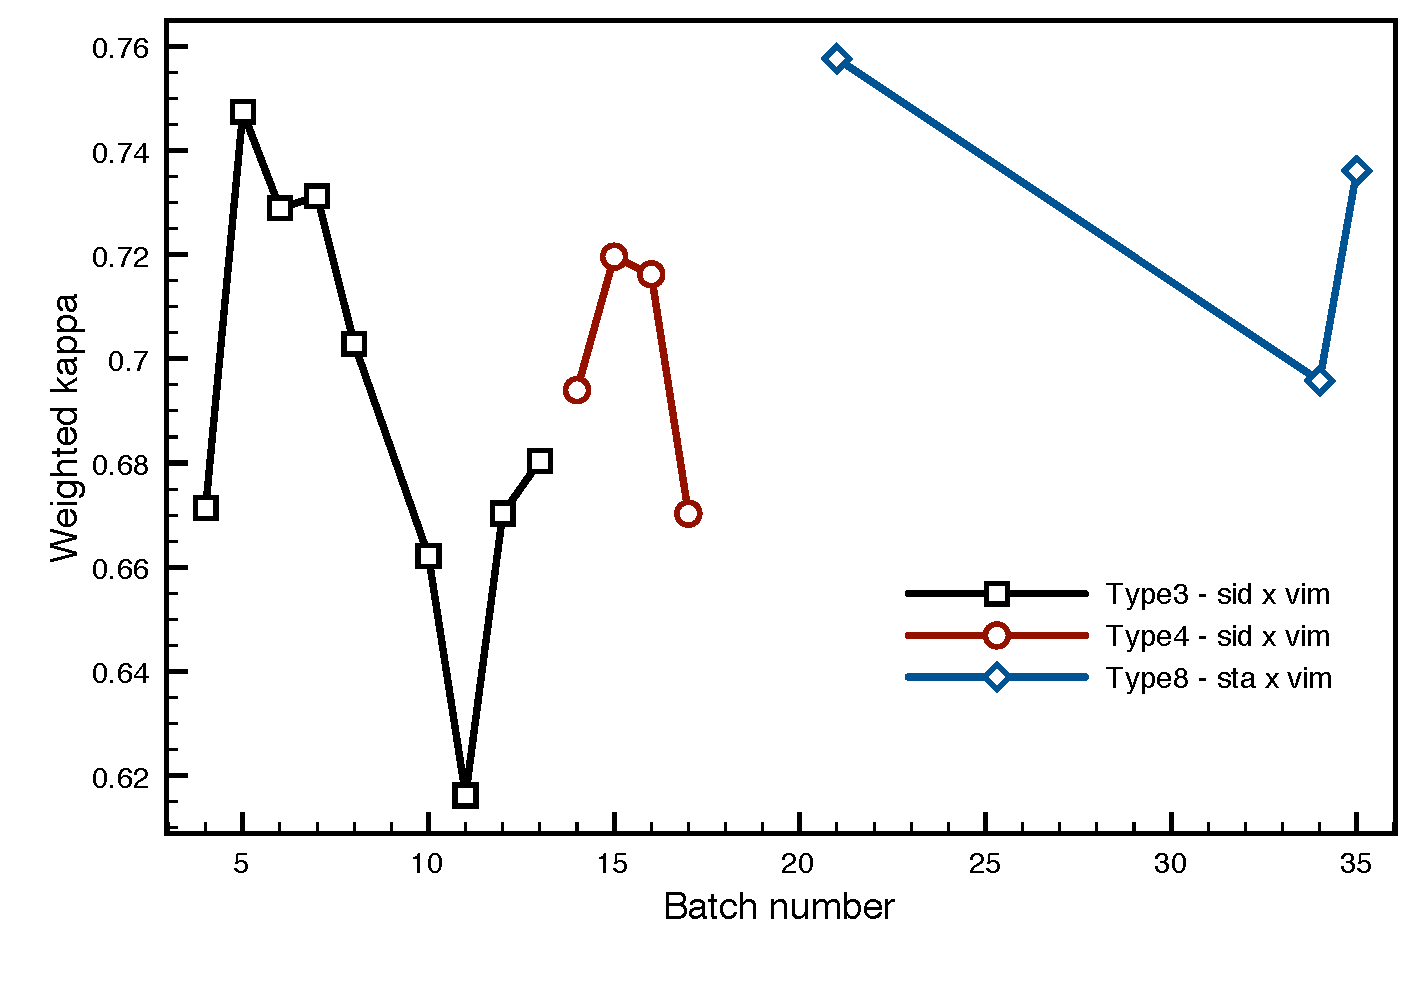
\includegraphics[width=\textwidth]{images/kappa.pdf}
   \caption{Weighted kappa per annotation type (colour line), a pair of annotators, and batches of annotated files (data points).}
   \label{fig:kappa}
\end{figure}
%%% tables and graphs for kappa_{w} -- END


We introduced improved $\kappa_w^U$ measure, which is weighted kappa with the upper bound moved from the value 1. This measure is the best fit for our problem that we were able to come up with. 

\subsection{Analysis of the disagreement}
When we analyse disagreement and partial agreement we find that most cases have to do with SemLex entries rather than NEs. This is mostly due to the deficiencies of the dictionary and its size (annotators could not explore each of almost 30,000 of SemLex entries). Our current methodology, which relies too much on searching the SemLex, is also to blame. This should, however, improve by employing pre-annotations (\ref{pre-static}) and (\ref{pre-on-load}). 

%\begin{compactitem}
%\item 
One more reason for disagreement consists in the fact that there are cases for which non-trivial knowledge of the world is needed: ``Jang Di Pertuan Agong Sultan Azlan Shah, the sultan of the state of Perak, [\kern 2pt \ldots] flew back to Perak.'' Is ``Sultan Azlan Shah'' still a part of the name or is it (or a part of it) a title?
%\item 

The last important cause of disagreement is simple: both annotators identify \emph{the same} part of text as MWE instances, but while searching the SemLex they choose different entry as the tags. This can be rectified by:
	\begin{compactitem}
		\item Removing duplicate entries from SemLex (currently there are many almost identical entries originating from Eurovoc and Czech WordNet).
		\item Imploring improved pre-annotation \ref{pre-static} and \ref{pre-on-load}, as mentioned above.
	\end{compactitem}
%\end{compactitem}
%\medskip

\xxx{We have recently begun annotations of pre-annota\-ted data (type \ref{pre-hnatkova}). If we may infer from such small data (319 lexias), this type of pre-annotation slightly helps on SemLex entries (it was the object of pre-annotation, from 34.7\% to 36.5\%) and slightly spoils the NE agreement (from 71.8\% to 67.1\%). Generally, on all lexias, it slightly improves agreement (from 58.2\% to 60.1\%). Speed improvement was quite noticeable, because vast majority of pre-annotated tags might be left untouched by annotators.}

\xxx{ k PI:\\
nase Max. je zalozene na predpokladu, ze data budou nadale podobne a anotatori nezacnou naraz anotovat vyrazne vic. 
Max. je stanoveno tak, ze za predpokladu vyse anotator nemuze (a ani nema) Max. dosahnout. Jelikoz jde o prunik vsech anotovanych uzlu, jsou v nem i chyby (v neshodach), ty ale kompenzuji pripadne uzly, ktere ani jeden neidentifikoval, ale meli.}

\section{Time analysis}
\label{sec:time-analysis}
Logs are a source of valuable information that can provide an insight into what is actually going on during annotation. Analysis of logs together with s-files can help estimate the real cost of annotations, which we have done during annotations to some extent, by estimating speed of annotations \see{sec:time-analysis}. 
But the analysis can go further and, to formulate the problem in economic terms, try to examine in general what factors influence the price of a (correct) tag. What is the relation of speed, length of work intervals, time of day, order of processing of the file, and other factors? We give only a very brief glimpse of one of the factors -- speed of annotations in \Sref{sec:time-analysis}, but in our opinion thorough statistical analysis of log files is an important source of information also for future annotation projects.

One of the reasons to implement detailed logs of all the annotations \see{sec:logs} was to allow detailed analysis of the time aspect of annotations. By ``time aspect'' we do not mean just checking, how much it takes annotators to tag the data, even though this is an important information too. We wanted to make it possible to ask any number of questions: Is there correlation between annotation speed and frequency of work? Does the speed increase or decrease in long stretches of continuous work? In how long intervals do annotators tend to work? Is the number of tags per minute/hour more or less constant?  

In \Fref{fig:speed} we can see some inter- and -intra annotator variance in speed, but it seems there are some clear broad tendencies: annotators tend to have their own speed, as shown by the splines They also show different amount of variance in speed, epsecially annotator \emph{sid}'s speed is visibly more stable.

\begin{figure}[htbp]
   \centering
   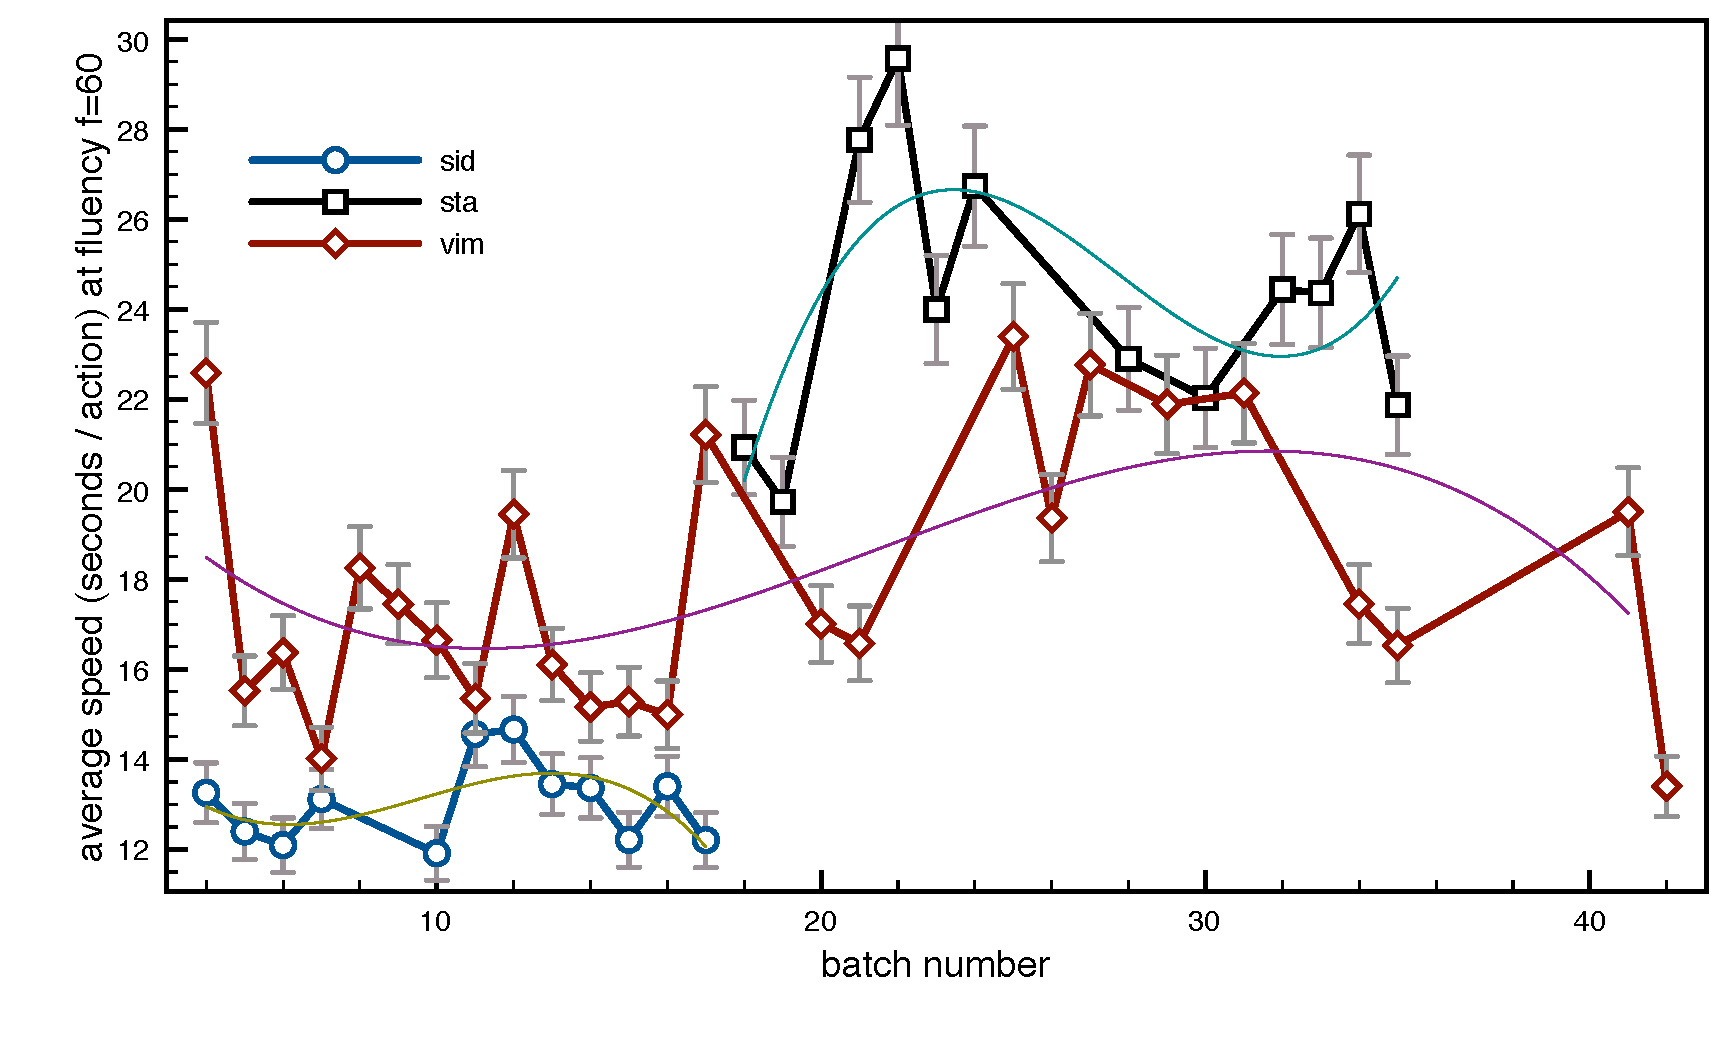
\includegraphics[width=\textwidth]{images/speed/speed-anot3} 
   \caption{Average speed of each annotator for each batch that he/she annotated. Grey vertical bars show 5\% error intervals.}
   \label{fig:speed}
\end{figure}



The data plotted in \Fref{fig:hist} and \Fref{fig:hist-detail}, even though not normalised to disregard the different amount of data annotated, shows remarkable similarity in behaviour of all three annotators.

\begin{figure}[htbp]
   \centering
   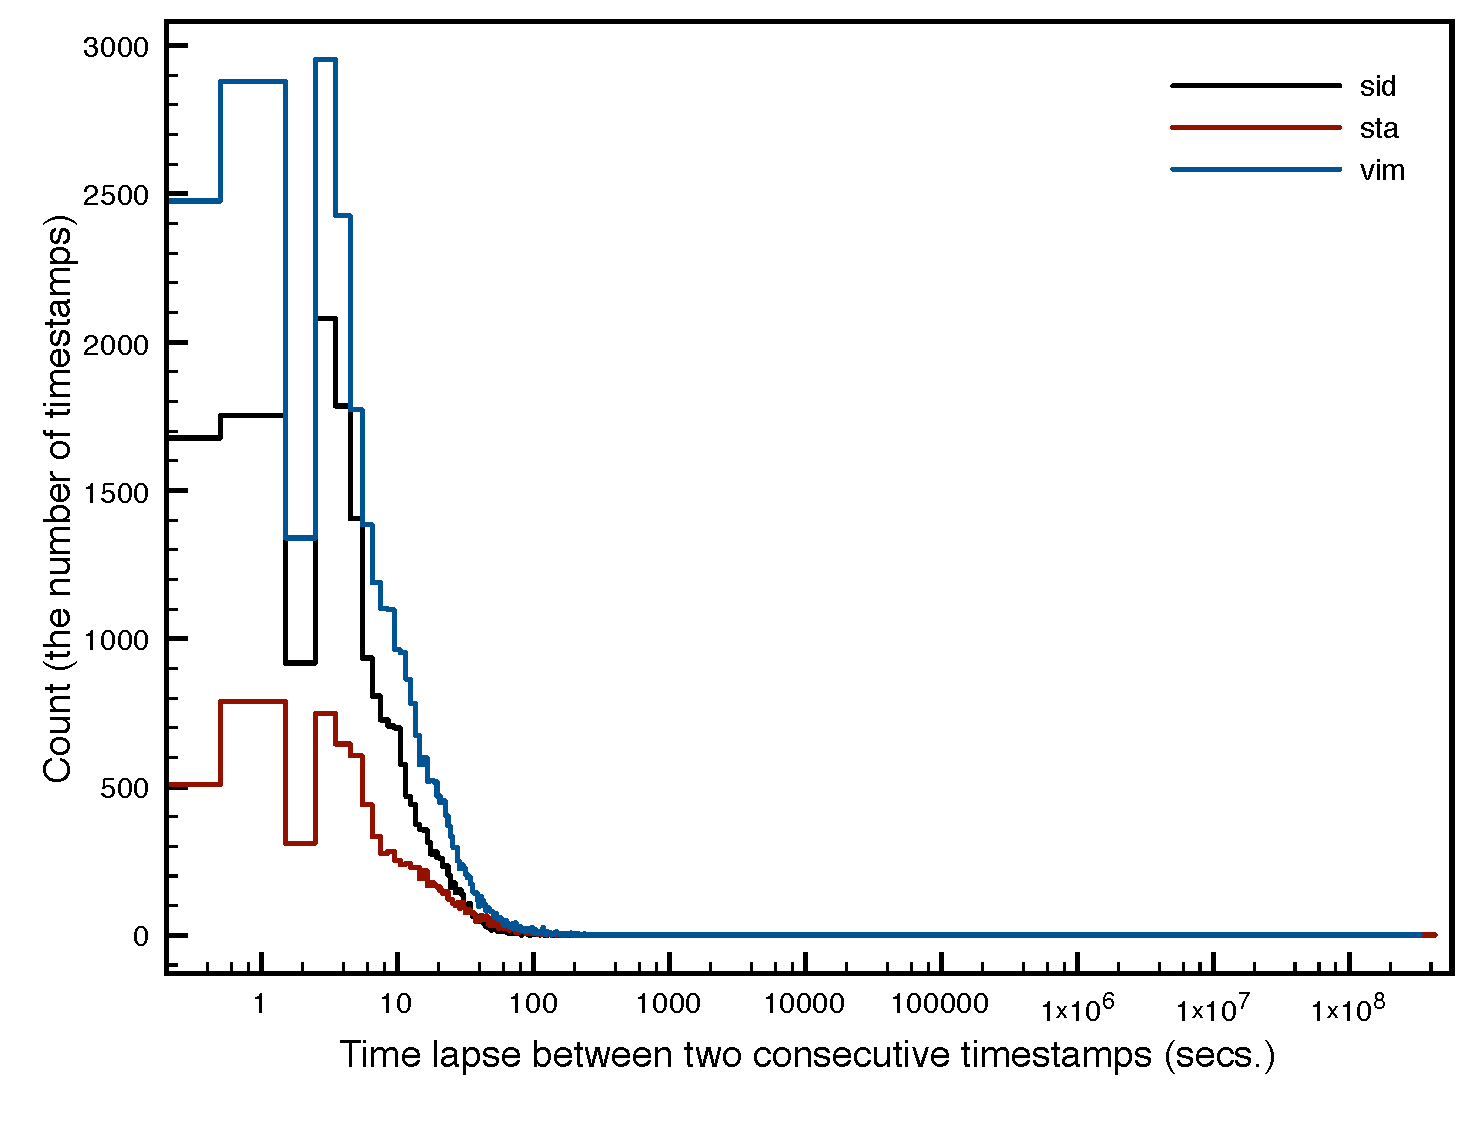
\includegraphics[width=.8\textwidth]{images/speed/histograms} 
   \caption{A histogram showing how many times ($y$) did an annotator place the next tag exactly $x$ seconds after the previous one.} 
   \label{fig:hist}
\end{figure}

\begin{figure}[htbp]
   \centering
   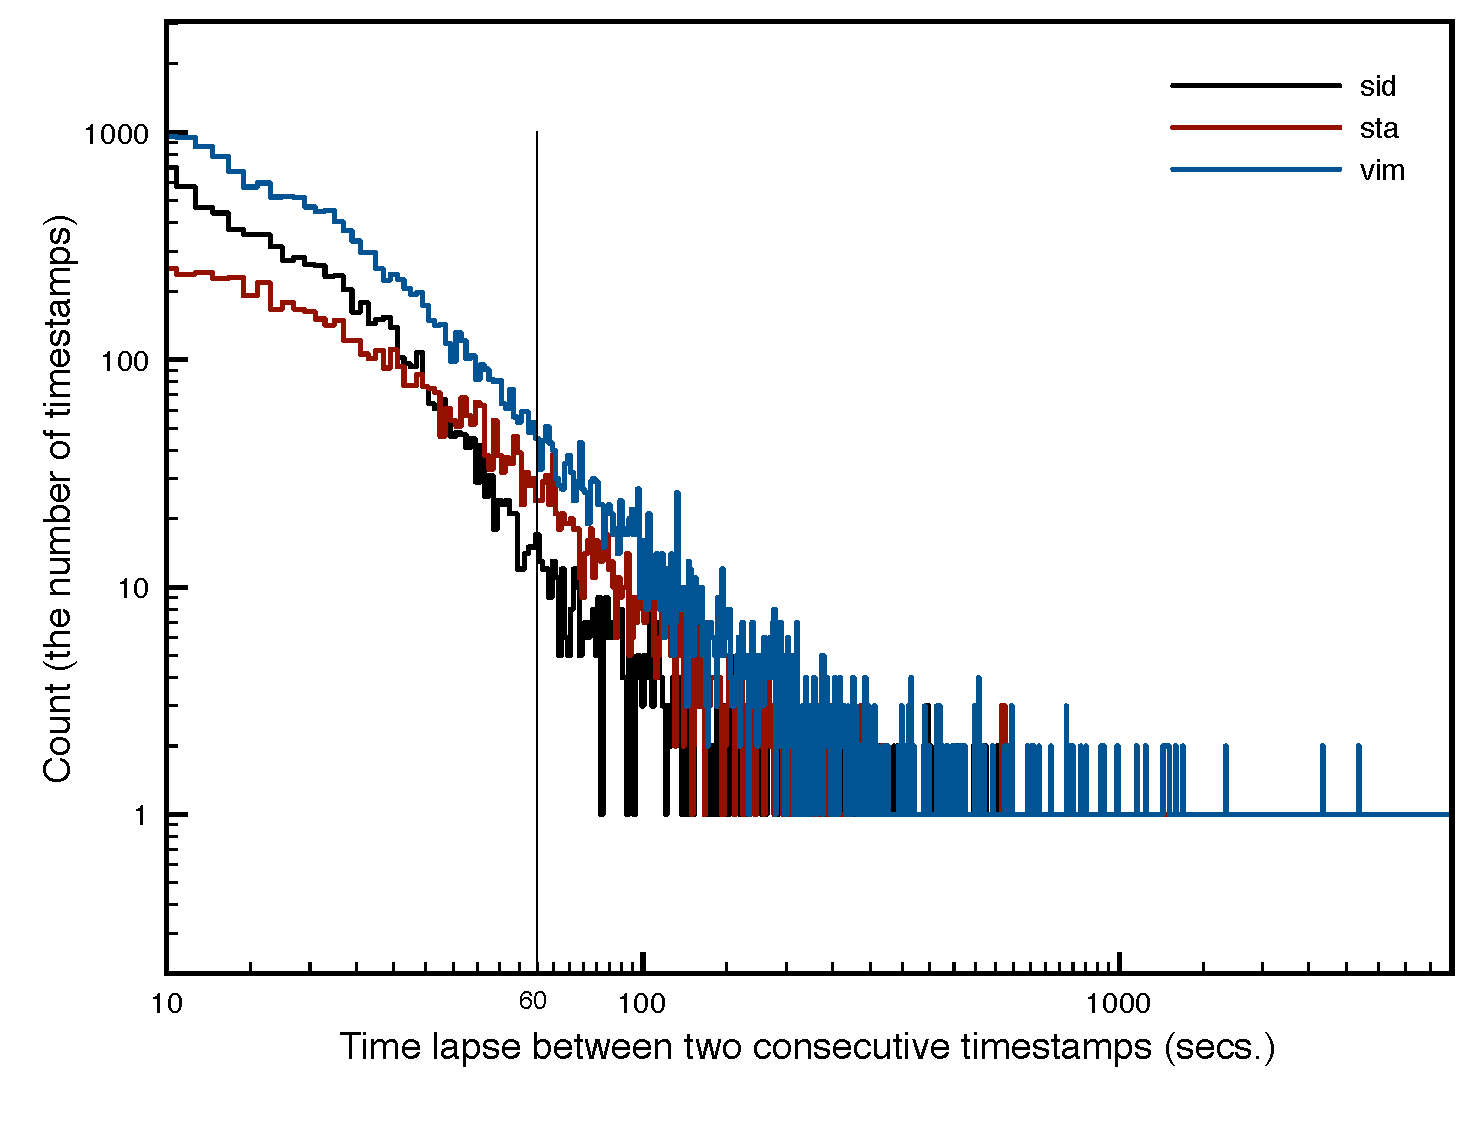
\includegraphics[width=.8\textwidth]{images/speed/histograms-detail} 
   \caption{Detail of the histogram in \Fref{fig:hist} in an interval where we have placed our \emph{fluency} value for the preliminary experiment with clustering of work into annotation intervals ($f=60$, see \Sref{sec:time-analysis} and \Fref{fig:speed}).}
\label{fig:hist-detail}
\end{figure}


\todo \xx{popsat analyzacni skript a fluency (f=60).}\\
\xxx{problem toho, co vlastne vidime, jak nastavit pocitani, nas skript, zakladni udaje, grafy}
